\chapter{Dwupętlowy regulator PID}
\label{thermal_pid}
Zasada działania dwupętlowego regulatora PID opiera się na wykorzystaniu dwóch niezależnych regulatorów PID. Dzięki takiemu rozwiązaniu możemy regulować obiekty $2x2$ (dwa wejścia i dwa wyjścia). Podejście to jest oczywiście skalowalne tzn. gdy będziemy mieli obiekt $4x4$ to użyjemy czterech regulatorów PID itd. 
\\ \indent W naszej implementacji zastosowaliśmy standardowe kroki używane podczas projektowania regulatorów wielowymiarowych w przemyśle:
\begin{enumerate}
\item Wybór wielkości sterujących $u_{1}$ i regulowanych $y_{i}$
\item Wybór struktury połączeń, wybieramy pary: wielkość regulowana - wielkość sterująca, które tworzą pojedyncze pętle sprzężenia zwrotnego 
\item Wybór rodzaju i strojenie nastaw regulatorów SISO (jednowymiarowych). 
\end{enumerate}
~\\ Z reguły strojenie tego typu regulatorów jest trudniejsze ponieważ nie może być dokonywane niezależnie. Nasze doświadczenia z strojeniem regulatora na stanowisku laboratoryjnym opiszemy w dalszych punktach. 

\section{Implementacja dwupętlowego regulatora PID na sterowniku PLC}
\label{thermal_pid_impl}
Do implementacji dwupętlowego regulatora PID użyliśmy języka ST, a za środowisko programistyczne posłużył nam program GX Works 3. Jest to dedykowane narzędzie do programowania sterowników PLC marki Mitsubishi. Piki z implementacją jednowymiarowych regulatorów PID znajdują się w folderze \textit{Fixed Scan}, który realizuje cykliczne przerwania. Nazwy tych plików to \textit{PID\_OUR\_1} i \textit{PID\_OUR\_2}.
\begin{lstlisting}[caption={Kod pierwszego jednowymiarowego regulatora PID}, language=C]
//Regulator PID_1 na podstawie rownania roznicowego
SV_PID1 := Zadana_PID1;
PV_PID1 := REAL_TO_INT(D100); // y_k ma byc zmienna okreslajaca pierwsze wyjscie z obiektu
//Wyliczenie parametrow
R0_PID1 := K_PID1*(1+(TP_PID1/(2*TI_PID1)) + TD_PID1/TP_PID1); //r0 = K*( 1+(Tp/(2*Ti))+Td/Tp );
R1_PID1 := K_PID1*( (TP_PID1/(2*TI_PID1)) - (2*TD_PID1/TP_PID1) - 1); //r1 = K*( (Tp/(2*Ti))-(2*Td/Tp)-1 );
R2_PID1 := K_PID1*TD_PID1/TP_PID1; //K*Td/Tp;
//Wyliczenie uchybu regulacji i przesuniecie historii
E2_PID1 := E1_PID1;
E1_PID1 := E0_PID1;
E0_PID1 := SV_PID1 - PV_PID1;

//Obliczenie sterowania
U_PID1 := R2_PID1*E2_PID1 + R1_PID1*E1_PID1 + R0_PID1*E0_PID1 + U_PID1;
//u = R2*E2 + R1*E1 + R0*E0 + u;

IF (U_PID1 > 1000.0) THEN
	U_PID1 := 1000;
END_IF;	
	
	
IF (U_PID1 < 0.0) THEN
	U_PID1 := 0.0;
	
	
END_IF;
\end{lstlisting}

\begin{lstlisting}[caption={Kod drugiego jednowymiarowego regulatora PID}, language=C]
//Regulator PID_2 na podstawie rownania roznicowego
SV_PID2 := Zadana_PID2;
PV_PID2 := REAL_TO_INT(D102); // y_k ma byc zmienna okreslajaca pierwsze wyjscie z obiektu 
//Wyliczenie parametrow
R0_PID2 := K_PID2*(1+(TP_PID2/(2*TI_PID2)) + TD_PID2/TP_PID2); //r0 = K*( 1+(Tp/(2*Ti))+Td/Tp );
R1_PID2 := K_PID2*( (TP_PID2/(2*TI_PID2)) - (2*TD_PID2/TP_PID2) - 1); //r1 = K*( (Tp/(2*Ti))-(2*Td/Tp)-1 );
R2_PID2 := K_PID2*TD_PID2/TP_PID2; //K*Td/Tp;
//Wyliczenie uchybu regulacji i przesuniecie historii
E2_PID2 := E1_PID2;
E1_PID2 := E0_PID2;
E0_PID2 := SV_PID2 - PV_PID2;

//Obliczenie sterowania
U_PID2 := R2_PID2*E2_PID2 + R1_PID2*E1_PID2 + R0_PID2*E0_PID2 + U_PID2;
//u = R2*E2 + R1*E1 + R0*E0 + u;

IF (U_PID2 > 1000.0) THEN
	U_PID2 := 1000.0;
END_IF;
IF (U_PID2 < 0.0) THEN
	U_PID2 := 0.0;
END_IF;

IF ( PV_PID2 > 15000) THEN
	U_PID2 := 0;
END_IF ;
\caption{Kod drugiego jednowymiarowego regulatora PID}
\end{lstlisting}

\begin{figure}[H]
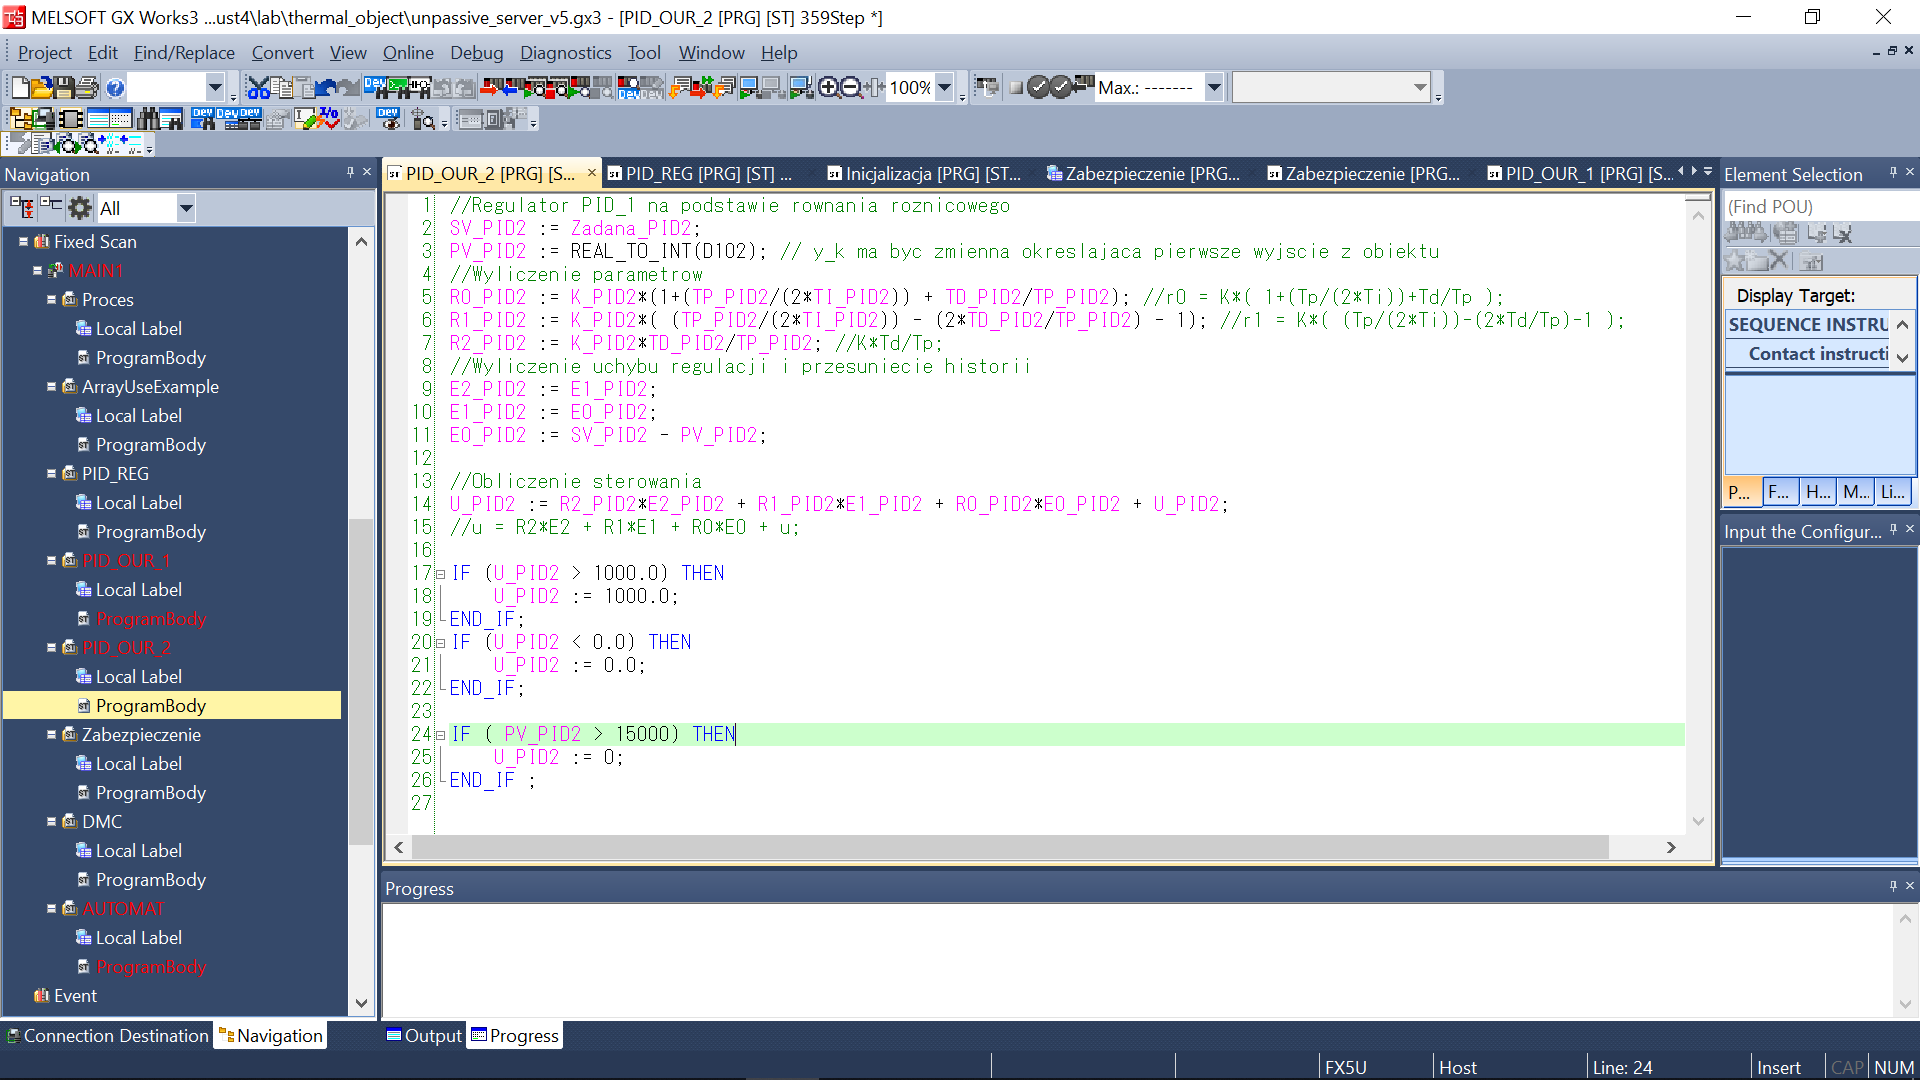
\includegraphics[scale=0.43]{sections/thermal/DrzewkoZFolderami.png}
\caption{Zrzut ekranu pokazujący strukturę elementu Fixed Scan}
\end{figure}


\section{Wyniki działania algorytmu regulacji}
\label{thermal_pid_wyniki}

\subsection{Pierwsza próba}
\label{thermal_pid_proba_1}

\subsection{Druga próba}
\label{thermal_pid_proba_2}

\subsection{Trzecia próba}
\label{thermal_pid_proba_3}